%----------------------------------------------------------------------------   
\chapter{\bevezetes}
%----------------------------------------------------------------------------

Napjainkban nagyon fontossá váltak a VoIP hívások megléte ugyanis a COVID-19 által okozott
pandémia alatt nem lehetett különböző korlátozások miatt fizikailag találkozni 
ismerőseinkkel, illetve dolgozni vagy tanulni. Erre egy jó megoldást nyújtottak a VoIP 
alkalmazások melyek segítségével valós időben lehet megbeszéléseket, órákat vagy 
találkozókat tartani. Viszont ez a megnövekedett használat megnövelte a alkalmazások 
által használt szerverek számát, amik még nem felhős környezetben futnak. A szakdolgozat 
hátralévő részében egy olyan megoldás kerül kifejtésre, ami lehetővé teszi, hogy az ezen 
rendszerekben használt RTP proxy szerver egy Kubernetes környezetben kerüljön 
felhasználásra. 

A hagyományos VoIP (Voice Over IP) hálózatok általában három részből állnak.
Az első rész, ami egyértelmű a kliensek, akik a hívásokat kezdeményezik és 
fogadják őket. A második maga a SIP (Session Initiation Protocol) szerver, aminek
az a dolga, hogy a kliensek által kapott SIP üzeneteket feldolgozza és ezek alapján
megfelelően állítsa be a harmadik elemet, ami egy RTP (Real-time Transport Protocol) 
proxy. Erre az proxyra azért van szükség, hogy irányítani és transzformálni lehessen az 
áthaladó forgalmat. Az \ref{fig:tradVoIP} ábrán látható egy ilyen rendszer egyszerűsített 
rajza.

\begin{figure}[!ht]
	\centering
	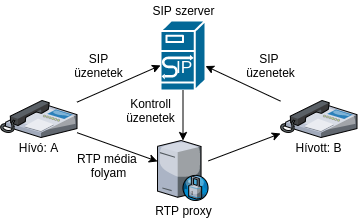
\includegraphics[width=0.5\textwidth, keepaspectratio]{figures/traditional_voip.png}
	\caption{Hagyományos VoIP hálózat}
	\label{fig:tradVoIP}
\end{figure}

Az \ref{fig:tradVoIP} ábrán egy általános hívásfelépítés látszik, ahol \textbf{A} hívja 
\textbf{B}-t. 
Ehhez, viszont SIP üzenetekben közölniük kell a SIP szerverrel, hogy ki milyen 
médiaformátumokat fogad el, melyik porton szeretnének kommunikálni és további hívással kapcsolatos információkat. A későbbiekben az összes ilyen protokoll kifejtésre fog
kerülni, hogy könnyebben látható legyen melyikre miért van szükség. Ha a SIP szerver
az összes üzenetet megkapta ahhoz, hogy létre tudjon hozni egy hívást, akkor az 
RTP proxynak megmondja, hogy hozzon létre egy hívást. Ha sikeresen létrejött a 
hívás, akkor kinyit két-két portot a hívásban résztvevő feleknek, amikre érkezhet
az adatfolyam. Azért nyit ki kettő portot kliensenként, mert az egyiken a
beszédmintákat illetve videó-képkockákat tartalmazó RTP csomagokat fogja
kezelni, míg a másikon a mádiaátvitel időzítését és statisztikázását szolgáló
RTCP (Real-time Transport Control Protocol) csomagokat küldi és fogadja. Mindezek mellett 
képes formátum konverziót is végrehajtani. Így ha a hívásban lévő két fél nem rendelkezik 
közös kódolási technikával, akkor is tudnak beszélgetni, mert az RTP proxy átfordítja 
mindkét félnek olyan kódolásra, amit képesek használni.

Ezzel a felépítéssel az a probléma, hogy az RTP proxy nem tud végtelen mennyiségű
hívást kezelni szabad port vagy erőforrás hiánya miatt. Emellett könnyen elérhetetlenné 
is válhat különböző fizikai tényezők miatt, mint erőforráshiány vagy hálózati eszközök 
meghibásodása végett. Így muszáj több példányt telepíteni a hálózatba, ami jelentősen 
megbonyolítja a rendszer karbantarthatóságát és új problémákat idéz elő. A munkám során
nem kerül megoldásra minden probléma, ami felmerülhet. A fókuszban ennek rendszernek az
olyan megvalósítása lesz melynek során úgy tud viselkedni a Kubernetes fürtben lévő
RTP proxy, mint egy erre a célra dedikált szerver.

A rugalmasság problémája fog megoldódni ebben a szakdolgozatban, ami az egy-egy RTP proxy
leállása során biztosítja az elérhetőséget a kliensek számára. Eredményül, ha az egyik
RTP proxy valamilyen oknál fogva megáll és nem képes további és meglévő kapcsolatait 
kiszolgálni, akkor egy másik RTP proxy példány képes egy Redis adatbázisból átvenni
a híváshoz szükséges információkat, amik alapján képes a megállt RTP proxy hívásainak
kezelését folytatni. 

Célom annak elérése, hogy az RTP proxy képes legyen Kubernetes rendszer alatt 
működni. De ehhez szükséges használni egy olyan szolgáltatáshálót, mint az L7mp. Ugyanis 
valahogyan kezelni kell a folyamatos UDP (User Datagram Protocol) forgalmat, amire
a jelenlegi szolgáltatáshálók közül kevesen képesek.

Ezenfelül kell egy kontroller, ami képes lesz hidat képezni az L7mp és az RTP proxy 
között. Erre azért van szükség, mert az L7mp nem képes automatikusan létrehozni a 
megfelelő forgalmi szabályokat. Ilyen szabályok szükségesek ahhoz, hogy egy hívás alatt a 
forgalom mindig ugyanahhoz az RTP proxyhoz érkezzen és ne összevissza a többi példány 
között.  

\begin{figure}[H]
	\centering
	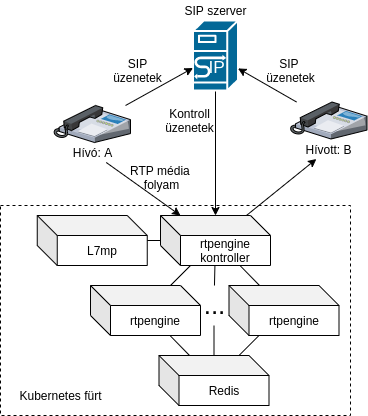
\includegraphics[width=0.55\textwidth,keepaspectratio]{figures/extended_traditional_voip.png}
	\caption{Módosított VoIP hálózat vázlatos felépítése}
	\label{fig:extVoIP}
\end{figure}

Az \ref{fig:extVoIP} ábrán látszik, hogy az RTP proxyt az rtpengine fogja megvalósítani
melyek Kubernetes kapszulákban kerülnek létrehozásra ezáltal biztosítva a skálázhatóságot
és a magas szintű elérhetőséget. Ezenfelül megjelenik az ábrán az L7mp, ami beérkező 
csomagokat fogja továbbítani a kontroller és az rtpengine-t futtató kapszulákhoz. Ennek
a két komponensnek az összekötését valósítja meg a kontroller, ami a beérkező üzenetek 
alapján képes az rtpengine-ben és az L7mp-ben is létrehozni a megfelelő erőforrásokat.  

\section{Szakdolgozat felépítése}

%Elsőnek a rendszerben résztvevő elemeket fogom részletesen bemutatni, hogy 
%tágabb rálátást lehessen nyerni ezekre a technológiákra. Majd részletesebben 
%foglalkozok azzal, hogy a hagyományos rendszer alatt hogyan működik egy hívás 
%kezelése. Erre azért van szükség, mert az új rendszerben is pontosan ugyanígy fog 
%működni, viszont az RTP proxy már nem csak egy egyszerű szerver lesz. 
%Ezután a felépített rendszerről lesz részletesebben információ és arról, hogy a
%kontroller hogyan működik ebben az egész megvalósításban. Amihez a használt
%klienst is befogom mutatni, mert azzal közvetlen lehet kommunikálni az RTP proxyval
%és tetszőleges számú hívás indítható el párhuzamosan. Végezetül pedig 
%a tesztek értékelése lesz és összehasonlítása az új és a régi rendszer között.

A szakdolgozat első részében bemutatásra kerülnek a híváshoz elengedhetetlen komponensek. 
Ebben részben látható lesz egy teljes értékű hagyományos hívás lebonyolítása is. Ebben a 
hagyományos hívásban még nem Kubernetes fürtben fog megjelenni az rtpengine. 

Bemutatásra kerül a létrehozott architektúra, melynek ismertetve lesz a fizikai háttere, 
ami a használt szerverek összeköttetését illetve azok telepítését írja le. Ismertetésre 
kerül, hogy az rtpengine, L7mp szolgáltatásháló és a kontroller miképp kerül 
összeköttetésbe egy Kubernetes fürtben. 

A tesztelésekhez tervezett kliensről is szó fog kerülni, ami közvetlen képes kommunikálni 
az rtpengine vezérlőprotokollján, így a SIP szervert megkerülve lehet hívásokat 
kezdeményezni. Ez a kliens nem egy teljes értékű VoIP kliens, mert csak a 
vezérlőprotokollt tudja használni híváskezdeményezésre. Illetve nem képes a hívások 
monitorozásához szükséges RTCP jelentéseket gyártani. 

Végezetül a mérések eredményei lesznek közölve és értékelve. Értékelve lesz a rendszer 
által nyújtott hívásminőség adott hívásmennyiség mellett és értékelésre kerül a rendszer 
rugalmassága is, melynek során vizsgálatra kerül, hogy mi történik akkor, amikor egy a 
hívást kezelő rtpengine kapszula kerül törlésre ezzel szimulálva a meghibásodást.

A megvalósított kontroller és kliens a \cite{repo} Github táróban elérhető a használt Kubernetes erőforrásokkal együtt. 